\documentclass[a4paper,onecolumn,oneside,12pt,extrafontsizes]{memoir}

%\usepackage[cp1250]{inputenc}
\usepackage[utf8]{inputenc}
\usepackage[T1]{fontenc}

\usepackage[polish]{babel}

\usepackage{setspace}

\usepackage{tabularx}

\usepackage{color,calc}
\usepackage{ebgaramond} 
\usepackage{tgtermes} 
\renewcommand*\ttdefault{txtt}

\usepackage{listings} 		% pakiet do prezentacji kodu. 

\clubpenalty=10000			%kara za sierotki
\widowpenalty=10000			% nie pozostawiaj wdów
\brokenpenalty=10000		% nie dziel wyrazów między stronami
\exhyphenpenalty=999999		% nie dziel słów z myślnikiem
\righthyphenmin=3			% dziel minimum 3 litery

\renewcommand{\topfraction}{0.95}
\renewcommand{\bottomfraction}{0.95}
\renewcommand{\textfraction}{0.05}
\renewcommand{\floatpagefraction}{0.35}

\usepackage{todonotes}

%%%%%%%%%%%%%%%%%%%%%%%%%%%%%%%%%%%%%%%%%%%%%%%%%%%

%%  Ustawienia rozmiarów: tekstu, nagłówka i stopki, marginesów

%%  dla dokumentów klasy memoir

%%%%%%%%%%%%%%%%%%%%%%%%%%%%%%%%%%%%%%%%%%%%%%%%%%%

\setlength{\headsep}{10pt}
\setlength{\headheight}{13.6pt} % wartość baselineskip dla czcionki 11pt tj. \small wynosi 13.6pt
\setlength{\footskip}{\headsep+\headheight}
\setlength{\uppermargin}{\headheight+\headsep+1cm}
\setlength{\textheight}{\paperheight-\uppermargin-\footskip-1.5cm}
\setlength{\textwidth}{\paperwidth-5cm}
\setlength{\spinemargin}{2.5cm}
\setlength{\foremargin}{2.5cm}
\setlength{\marginparsep}{2mm}
\setlength{\marginparwidth}{2.3mm}
\checkandfixthelayout[fixed] % konieczne, aby się dobrze wszystko poustawiało

%%%%%%%%%%%%%%%%%%%%%%%%%%%%%%%%%%%%%%%%%%%%%%%%

%%  Ustawienia odległości linii, wcięć, odstępów

%%%%%%%%%%%%%%%%%%%%%%%%%%%%%%%%%%%%%%%%%%%%%%%%

\linespread{1}
\setlength{\parindent}{14.5pt}

%%%%%%%%%%%%%%%%%%%%%%%%%%%%%%%%%%%%%%%%%%%%%%%%%%%

%%  Pakiety i komendy zastosowane tylko do zamieszczenia informacji o użytych komendach i fontach

%%  Normalnie nie są potrzebne, można je zamarkować podczas redakcji pracy

%%%%%%%%%%%%%%%%%%%%%%%%%%%%%%%%%%%%%%%%%%%%%%%%%%%

%\usepackage{memlays}     % extra layout diagrams, zastosowane w szblonie do 'debuggowania', używa pakietu layouts
\usepackage{printlen} % pakiet do wyświetlania wartości zdefiniowanych długości, stosowany do 'debuggowania'
\uselengthunit{pt}
\makeatletter
\newcommand{\showFontSize}{\f@size pt} % makro wypisujące wielkość bieżącej czcionki
\makeatother

% do pokazania ramek można byłoby użyć:
%\usepackage{showframe}

%%%%%%%%%%%%%%%%%%%%%%%%%%%%%%%%%%%%%%%%%%%%%%%%%%%

%%  Formatowanie list wyliczeniowych, wypunktowań i własnych otoczeń

%%%%%%%%%%%%%%%%%%%%%%%%%%%%%%%%%%%%%%%%%%%%%%%%%%%


\usepackage{enumitem} % pakiet pozwalający zarządzać formatowaniem list wyliczeniowych
\setlist{noitemsep,topsep=4pt,parsep=0pt,partopsep=4pt,leftmargin=*} % zadeklarowane parametry pozwalają uzyskać 'zwartą' postać wypunktowania bądź wyliczenia
\setenumerate{labelindent=0pt,itemindent=0pt,leftmargin=!,label=\arabic*.} % można zmienić \arabic na \alph, jeśli wyliczenia mają być z literkami
\setlistdepth{4} % definiujemy głębokość zagnieżdżenia list wyliczeniowych do 4 poziomów
\setlist[itemize,1]{label=$\bullet$}  % definiujemy, jaki symbol ma być użyty w wyliczeniu na danym poziomie
\setlist[itemize,2]{label=\normalfont\bfseries\textendash}
\setlist[itemize,3]{label=$\ast$}
\setlist[itemize,4]{label=$\cdot$}
\renewlist{itemize}{itemize}{4}

\makeatletter
\renewenvironment{quote}{
\begin{list}{}
{
\setlength{\leftmargin}{1em}
\setlength{\topsep}{0pt}%
\setlength{\partopsep}{0pt}%
\setlength{\parskip}{0pt}%
\setlength{\parsep}{0pt}%
\setlength{\itemsep}{0pt}
}
}{
\end{list}}
\makeatother

%%%%%%%%%%%%%%%%%%%%%%%%%%%%%%%%%%%%%%%%%

%%  Pakiet do generowania indeksu (ważne, aby wstawić przed hyperref)

%%%%%%%%%%%%%%%%%%%%%%%%%%%%%%%%%%%%%%%%%

\DisemulatePackage{imakeidx}
\usepackage[makeindex,noautomatic]{imakeidx} % tutaj mówimy, żeby indeks nie generował się automatycznie,
\makeindex
\makeatletter
\makeatother


\usepackage{ifpdf}
\ifpdf
	\usepackage[pdftex,bookmarks,breaklinks,unicode]{hyperref}
	\usepackage[pdftex]{graphicx}
	\DeclareGraphicsExtensions{.pdf,.jpg,.mps,.png}
\pdfcompresslevel=9
\pdfoutput=1
\makeatletter
\AtBeginDocument{
	\hypersetup{
		pdfinfo={
		Title = {\@title},
		Author = {\@author},
		Subject={},
		Keywords={słowa kluczowe},
		}
    }
}

\makeatother
\else
\usepackage{graphicx}
\DeclareGraphicsExtensions{.eps,.ps,.jpg,.mps,.png}
\fi
\sloppy

% Deklaracja głębokościu numeracji
\setcounter{secnumdepth}{2}
\setcounter{tocdepth}{2}
\setsecnumdepth{subsection} % activating subsubsec numbering in doc

% Kropki po numerach sekcji
\makeatletter
\def\@seccntformat#1{\csname the#1\endcsname.\quad}
\def\numberline#1{\hb@xt@\@tempdima{#1\if&#1&\else.\fi\hfil}}
\makeatother

\renewcommand{\chapternumberline}[1]{#1.\quad}
\renewcommand{\cftchapterdotsep}{\cftdotsep}

% Czcionka do podpisów tabel i rysunków
\captionnamefont{\small}
\captiontitlefont{\small}

% Przedefiniowanie etykiet w podpisach tabel i rysunków
%\AtBeginDocument{%
    \addto\captionspolish{%
    \renewcommand{\tablename}{Tab.}%
}%}

%\AtBeginDocument{%
    \addto\captionspolish{%
    \renewcommand{\figurename}{Rys.}%
}%}

%\AtBeginDocument{%
    \addto\captionspolish{%
    \renewcommand{\bibname}{Literatura}%
}%}

%\AtBeginDocument{%
    \addto\captionspolish{%
    \renewcommand{\listfigurename}{Spis rysunków}%
}%}

%\AtBeginDocument{%
    \addto\captionspolish{%
    \renewcommand{\listtablename}{Spis tabel}%
}%}

%\AtBeginDocument{%
    \addto\captionspolish

%%%%%%%%%%%%%%%%%%%%%%%%%%%%%%%%%%%%%%%%%%%%%%%%%%%%%%%%%%%%%%%%%%

%% Definicje stopek i nagłówków

%%%%%%%%%%%%%%%%%%%%%%%%%%%%%%%%%%%%%%%%%%%%%%%%%%%%%%%%%%%%%%%%%%

\addtopsmarks{headings}{%
\nouppercaseheads % added at the beginning
}{%

\createmark{chapter}{both}{shownumber}{}{. \space}
%\createmark{chapter}{left}{shownumber}{}{. \space}
\createmark{section}{right}{shownumber}{}{. \space}
}%use the new settings

\makeatletter
\copypagestyle{outer}{headings}
\makeoddhead{outer}{}{}{\small\itshape\rightmark}
\makeevenhead{outer}{\small\itshape\leftmark}{}{}
\makeoddfoot{outer}{\small\@author:~\@titleShort}{}{\small\thepage}
\makeevenfoot{outer}{\small\thepage}{}{\small\@author:~\@title}
\makeheadrule{outer}{\linewidth}{\normalrulethickness}
\makefootrule{outer}{\linewidth}{\normalrulethickness}{2pt}
\makeatother

% fix plain
\copypagestyle{plain}{headings} % overwrite plain with outer
\makeoddhead{plain}{}{}{} % remove right header
\makeevenhead{plain}{}{}{} % remove left header
\makeevenfoot{plain}{}{}{}
\makeoddfoot{plain}{}{}{}

\copypagestyle{empty}{headings} % overwrite plain with outer
\makeoddhead{empty}{}{}{} % remove right header
\makeevenhead{empty}{}{}{} % remove left header
\makeevenfoot{empty}{}{}{}
\makeoddfoot{empty}{}{}{}



%%%%%%%%%%%%%%%%%%%%%%%%%%%%%%%%%%%%%%%

%% Definicja strony tytułowej

%%%%%%%%%%%%%%%%%%%%%%%%%%%%%%%%%%%%%%%
\makeatletter
%Uczelnia
\newcommand\uczelnia[1]{\renewcommand\@uczelnia{#1}}
\newcommand\@uczelnia{}

%Wydział
\newcommand\wydzial[1]{\renewcommand\@wydzial{#1}}
\newcommand\@wydzial{}

%Kierunek
\newcommand\kierunek[1]{\renewcommand\@kierunek{#1}}
\newcommand\@kierunek{}

%Specjalność
\newcommand\specjalnosc[1]{\renewcommand\@specjalnosc{#1}}
\newcommand\@specjalnosc{}

%Tytuł po angielsku
\newcommand\titleEN[1]{\renewcommand\@titleEN{#1}}
\newcommand\@titleEN{}

%Tytuł krótki

\newcommand\titleShort[1]{\renewcommand\@titleShort{#1}}
\newcommand\@titleShort{}

%Promotor
\newcommand\promotor[1]{\renewcommand\@promotor{#1}}
\newcommand\@promotor{}


\usepackage[absolute]{textpos} % zamarkowano, bo ostatecznie wykorzystano otoczenie picture


\def\maketitle{%
    \pagestyle{empty}%
%%\garamond
    \fontfamily{\ebgaramond@family}\selectfont % na stronie tytułowej czcionka garamond
%%%%%%%%%%%%%%%%%%%%%%%%%%%%%%%%%%%%%
%% Poniżej, w otoczniu picture, wstawiono tytuł i autora.
%% Tytuł (z autorem) musi znaleźć się w obszarze
%% odpowiadającym okienku 110mmx75mm, którego lewy górny róg
%% jest w położeniu 77mm od lewej i 111mm od górnej  krawędzi strony
%% (tak wynika z wycięcia na okładce).
%% Poniższy kod musi być użyty dokładnie w miejscu gdzie jest.
%% Jeśli tytuł nie mieści się w okienku, to należy tak pozmieniać
%% parametry użytych komend, aby ten przydługi tytuł jednak
%% upakować go do okienka.
%%

%% Sama okładka (kolorowa strona z wycięciem, do pobrania z dydaktyki)
%% powinna być przycięta o 3mm od każdej z krawędzi.
%% Te 3mm pewnie zostawiono na ewentualne spady czy też specjalną oprawę.
%%%%%%%%%%%%%%%%%%%%%%%%%%%%%%%%%%%%%

    \newlength{\tmpfboxrule}
    \setlength{\tmpfboxrule}{\fboxrule}
    \setlength{\fboxsep}{2mm}
    \setlength{\fboxrule}{0mm}
    %\setlength{\fboxrule}{0.1mm} %% jeśli chcemy zobaczyć ramkę
    \setlength{\unitlength}{1mm}

    \begin{picture}(0,0)
\put(26,-124){\fbox{
    \parbox[c][71mm][c]{104mm}{\centering
    {\fontsize{16pt}{18pt}\selectfont \@title}\\[5mm]
    {\fontsize{16pt}{18pt}\selectfont \@titleEN}\\[20mm]
    {\fontsize{16pt}{18pt}\selectfont AUTOR:}\\[2mm]
    {\fontsize{14pt}{16pt}\selectfont \@author}}
}
}
\end{picture}

\setlength{\fboxrule}{\tmpfboxrule}
%%%%%%%%%%%%%%%%%%%%%%%%%%%%%%%%%%%%%

%% Reszta strony z nazwą uczelni, wydziału, kierunkiem, specjalnością
%% promotorem, oceną pracy, miastem i rokiem
{\centering%\vspace{-1cm}
{\fontsize{22pt}{24pt}\selectfont \@uczelnia}\\[0.4cm]
{\fontsize{22pt}{24pt}\selectfont \@wydzial}\\[0.5cm]
\hrule %\vspace*{0.7cm}
}

{\flushleft\fontsize{14pt}{16pt}\selectfont%
\begin{tabular}{ll}
KIERUNEK: & \@kierunek\\
SPECJALNOŚĆ: & \@specjalnosc\\
\end{tabular}\\[1.3cm]
}

{\centering
{\fontsize{32pt}{36pt}\selectfont PRACA}\\[0.5cm]
{\fontsize{32pt}{36pt}\selectfont INŻYNIERSKA}\\[2.5cm]
}

\vfill

\begin{tabularx}{\linewidth}{p{6cm}l}
&{\fontsize{16pt}{18pt}\selectfont PROWADZĄCY PRACĘ:}\\[2mm] %UWAGA: tutaj jest miejsce na nazwisko promotora pracy
&{\fontsize{14pt}{16pt}\selectfont \@promotor}\\[10mm]
&{\fontsize{16pt}{18pt}\selectfont OCENA PRACY:}\\[20mm]

\end{tabularx}

\vspace{2cm}
\hrule\vspace*{0.3cm}
{\centering
{\fontsize{16pt}{18pt}\selectfont \@date}\\[0cm]
}

%\ungaramond
\normalfont
    \cleardoublepage
}
\makeatother
%%%%%%%%%%%%%%%%%%%%%%%%%%%%%%%%%%%%%%%%%


%%%%%%%%%%%%%%%%%%%%%%%%%%%%%%%%%%%%%%%%%

%%  Metadane dokumentu

%%%%%%%%%%%%%%%%%%%%%%%%%%%%%%%%%%%%%%%%%

\title{Zarządzanie zadaniami w systemie obrazowania wielospektralnego}
\titleShort{Zarządzanie zadaniami ...}
\titleEN{Task management for hyperspectral imaging system}
\author{Aleksander Cieślak}
\uczelnia{POLITECHNIKA WROCŁAWSKA}
\wydzial{WYDZIAŁ ELEKTRONIKI}
\kierunek{INFORMATYKA}
\specjalnosc{INŻYNIERIA SYSTEMÓW INFORMATYCZNYCH}
\promotor{dr inż. Tadeusz Tomczak}
\date{WROCŁAW, \today}

\begin{document}

% Tutaj można przełączyć odstęp między liniami
\SingleSpacing
%\OnehalfSpacing
%\DoubleSpacing

%\settypeoutlayoutunit{cm} % do debugowania
%\typeoutstandardlayout    % wypisuje na stdout informacje o ustawieniach
\maketitle

\newpage
\newpage

\chapterstyle{noNumbered}
\pagestyle{outer}
\mbox{}\pdfbookmark[0]{Spis treści}{spisTresci.1}
\tableofcontents*

\newpage
\mbox{}\pdfbookmark[0]{Spis rysunków}{spisRysunkow.1}
\listoffigures*
\begin{flushleft}
\end{flushleft}

\newpage
\mbox{}\pdfbookmark[0]{Spis tabel}{spisTabel.1}
\listoftables*

%\include{skroty} %skróty można sobie pominąć

\chapterstyle{default}

\chapter{Cel projektu}

Celem niniejszej pracy jest projekt i~implementacja modułu zarządzania zadaniami dla systemu Gerbil (\url{http://gerbilvis.org/}). Jest to system do analizy i~wizualizacji danych wielospektralnych. Gerbil posiada zestaw wielu algorytmów przetwarzania obrazów oraz uczenia maszynowego, które przekładają się na szerokie spektrum funkcjonalności. Jednak jego słabym punktem jest warstwa zarządzania danymi oraz potok przetwarzania danych. To z~kolei powoduje niestabilność całej aplikacji. W~ramach pracy dyplomowej został zaproponowany system, który rozwiązuje wyżej wspomniane problemy. System ten pozwala na bezpieczny dostęp do danych w~całej aplikacji oraz gwarantuje zachowanie właściwego potoku przetwarzania danych.
Kod źródłowy systemu można znaleźć pod adresem \url{https://github.com/ajaskier/gerbil/tree/distalpha}.


\chapter{Obrazowanie wielospektralne}
Obrazowanie wielospektralne jest techniką rejestracji obrazu za pomocą fal elektromagnetycznych o~wybranej częstotliwości spośród widma spektroskopowego. Podczas gdy ludzkie oko widzi głównie w trzech zakresach spektralnych (czerwonym, niebieskim oraz żółtym), obraz wielospektralny jest rejestrowany w znacznie większej liczbie zakresów (przykładowo 31).

\section{Format danych}
\index{kostka wielospektralna} Dane wielospektralne są często nazywane kostką wielospektralną. 

\begin{figure}[ht]
	\centering
		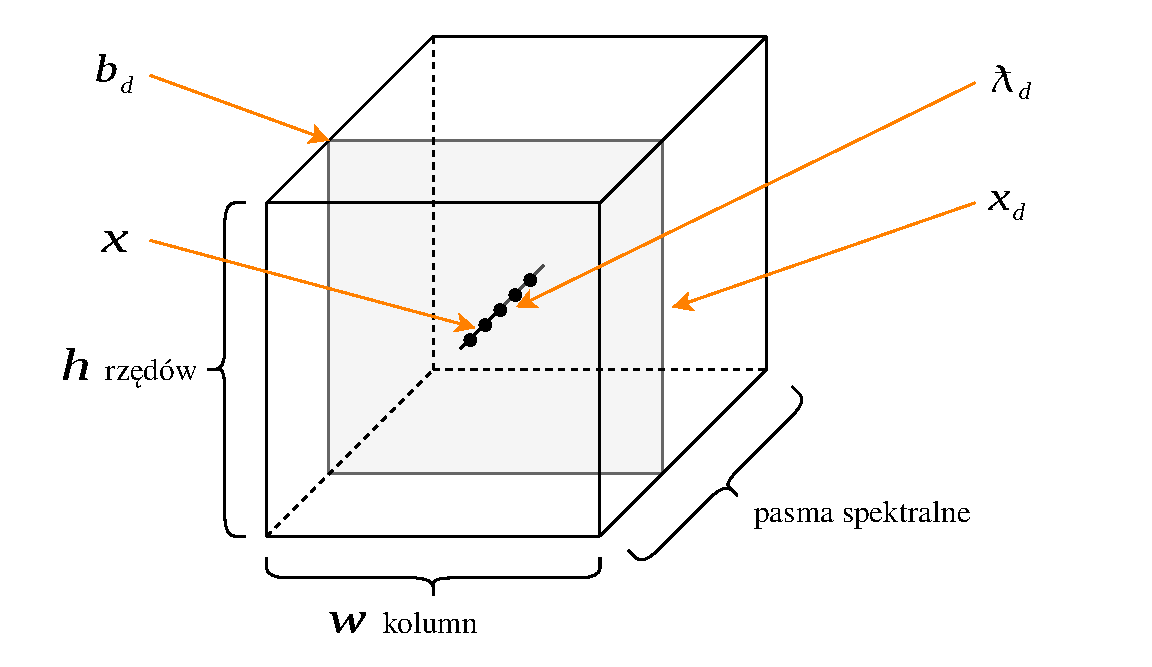
\includegraphics[width=0.75\linewidth]{rys02/multispectral-cube-vector}
	\caption{Schemat kostki wielospektralnego}
	\label{fig:multispectral-cube}	
\end{figure}

Na rysunku ~\ref{fig:multispectral-cube} zilustrowano układ danych w kostce wielospektralnej. Kostka taka składa się z~$n_x$ ($h$ rzędów na $w$ kolumn) pikseli $x$. Każdy piksel jest wektorem współczynników spektralnych o~długości  $n_D$, gdzie $n_D$ jest liczbą obrazów spektralnych, na które składa się dana wielospektralna. Każdy współczynnik $x_d$ jest wartością reakcji sensorycznej dla odpowiadającego pasma spektralnego $b_d$ skoncentrowanego wokół fali $\lambda_d$. W skrócie obraz wielospektralny jest zbiorem obrazów rejestrowanych przy użyciu fal elektromagnetycznych o~zadanych długościach. 


\subsection{Konsekwencje formatu danych}
Ze względu na swoją charakterystykę serie obrazów wielospektralnych mogą bezproblemowo osiągać rozmiary setek megabajtów, lub nawet gigabajtów. Zazwyczaj jednak obrazy są rejestrowane aparatem o~matrycy ok. 2 Mpix. Większość danych pochodnych, które są efektem analizy tego obrazu posiadają podobne rozmiary. Informacja ta jest kluczowa podczas projektowania mechanizmu zarządzania danymi w~takim systemie. Biorąc pod uwagę rozmiar danych mechanizm taki powinien:
\begin{itemize}
\item unikać tworzenia zbędnych kopi danych,
\item dokonywać obliczeń danych wyłącznie na żądanie,
\item zwalniać z~pamięci dane, które nie są już wykorzystywane przez aplikację.
\end{itemize}

\section{Dane w systemie Gerbil}

Oryginalny obraz wielospektralny jest traktowany jako dana wejściowa w systemie. Na jego podstawie powstają dane pochodne. Są to głównie kolejne obrazy oraz histogramy wielospektralne. Do stworzenia prototypu mechanizmu zarządzania danymi oraz procesem przetworzenia użyte zostały poniższe dane:
\begin{itemize}
	\item \index{image} \textbf{image} -- oryginalny obraz wielospektralny. Dana ta jest obliczana podczas inicjalizacji aplikacji. Użytkownik może wejść w interakcję z~systemem dopiero gdy image zostanie przetworzone.
	\item \index{ROI} \textbf{ROI (Region of Interest)} -- wyselekcjonowany podzbiór danych, w tym przypadku wybrane prostokątne zaznaczenie obrazu. Jest przechowywany jako współrzędne lewego górnego wierzchołka zaznaczenia, jego wysokość oraz szerokość,
	\item \index{image.IMG} \textbf{image.IMG} -- fragment obrazu oryginalnego zdeterminowany przez ROI,
	\item \index{image.NORM} \textbf{image.NORM} -- image.IMG po normalizacji wektorów składających się z~pikseli o~jednakowych współrzędnych na przestrzeni pasm spektralnych,
	\item \index{image.GRAD} \textbf{image.GRAD} -- gradient obrazu image.IMG,
	\item \index{image.PCA} \textbf{image.PCA} -- image.IMG po zastosowaniu metody PCA (analizy głównych składowych),
	\item \index{image.GRADPCA} \textbf{image.GRADPCA} -- image.GRAD po zastosowaniu metody PCA (ang. Principal Component Analysis - Analiza głównych składowych)\cite{PCA},
	\item \index{band} \textbf{bands.*.N} -- pojedynczy N-ty obraz spektralny danej reprezentacji image.* (przykładowo bands.NORM.6),
	\item \index{dist.IMG} \textbf{dist.IMG} - histogram wielospektralny obrazu image.IMG,
	\item \index{dist.tmp.IMG} \textbf{dist.tmp.IMG} - dana pomocnicza używana do uzyskania danej dist.IMG. 
\end{itemize}
Z racji, że jedne dane produkują inne, łatwo jest zdefiniować hierarchię danych w tym systemie.

\begin{figure}[ht]
	\centering
		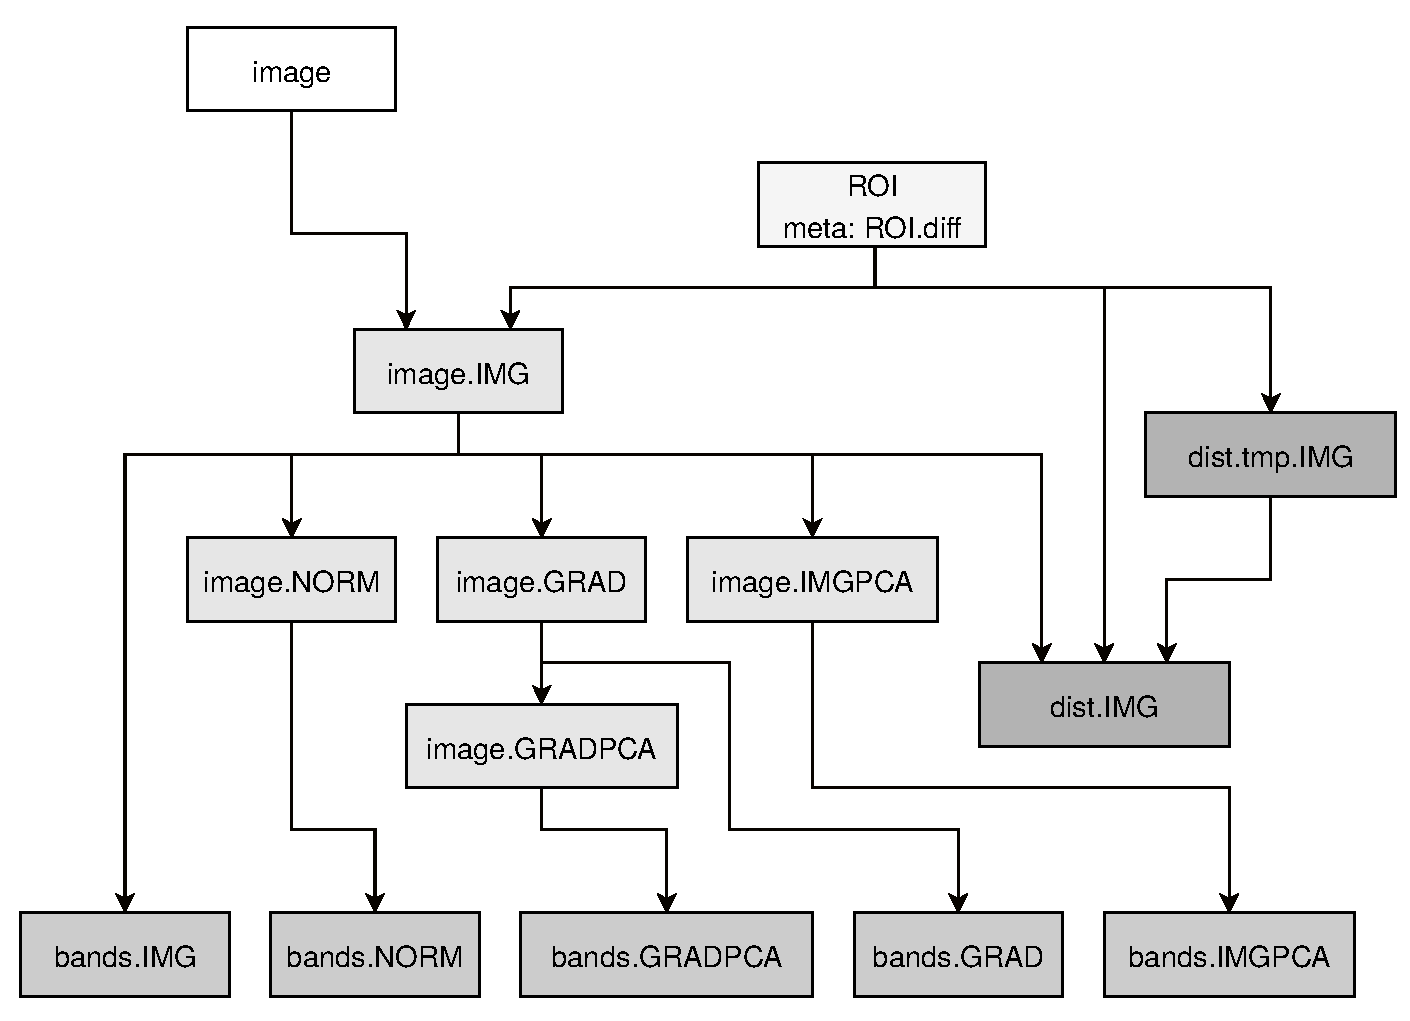
\includegraphics[width=0.7\linewidth]{rys02/data-dependencies}
	\caption{Graf zależności danych w systemie Gerbil}
	\label{fig:data-dependencies}	
\end{figure}

%\todo{Groty strzałek prawdopodobnie powinny być skierowane przeciwnie}
%\todo{Pojawiają się dziwne problemy z wstawieniem tego obrazka}

Na rysunku ~\ref{fig:data-dependencies} przedstawiono diagram zależności danych. Dane jednego koloru są do siebie semantycznie zbliżone. Przykładowo, image.NORM, image.GRAD, image.GRADPCA itp. są reprezentacjami obrazu oryginalnego. Dane posiadają również swoje metadane. Przykładowo metadaną ROI jest ROI.diff, które określa różnicę pomiędzy aktualnym a~poprzednim ROI. 

\subsection{Wpływ hierarchii danych na proces wykonania}
Analizując rysunek ~\ref{fig:data-dependencies} można dojść do wniosku, że proces przetworzenia danych jest dyktowany poprzez ich hierarchię. Przykładowo do obliczenia image.GRADPCA wymagane jest aby dane image, ROI, image.IMG oraz image.GRAD były już przetworzone. Dodatkowo można określić porządek, w którym te dane powinny zostać obliczone:

\begin{enumerate}[labelwidth=\widthof{\ref{last-item}},label=\arabic*.]
	\item image (podczas inicjalizacji systemu),
	\item ROI,
	\item image.IMG,
	\item image.GRAD,
	\item image.GRADPCA. \label{last-item}
\end{enumerate}

Scenariusz ten zakłada obliczenie każdej danej w hierarchii, co jest przypadkiem skrajnym. Często zdarza się, że pewna część danych jest aktualna. Wówczas przetwarzanie powinno rozpocząć się od pierwszej nieaktualnej danej znajdującej się najwyżej w hierarchii. 

Dodatkowo należy rozpatrzeć scenariusz równoległego wykonywania zadań. Zakładając, że aplikacja wyświetla jednocześnie dane image.NORM oraz image.GRAD, natomiast image.IMG zostało odświeżone, można dojść do wniosku, że system powinien w następnym kroku dokonać obliczeń obu danych (image.NORM i~image.GRAD). Obliczenia te można wykonać szeregowo bądź równolegle, wobec tego można zdefiniować opcjonalne wymaganie dla systemu zarządzania zadaniami jako możliwość równoległego przetwarzania zadań.

\bibliographystyle{plabbrv}

%UWAGA: bibliotekę referencji należy przygotować samemu. Dobrym do tego narzędziem jest JabRef.

%       Nazwę przygotowanej biblioteki wpisuje się poniżej bez rozszerzenia
%       (w tym przypadku jest to "dokumentacja.bib")

%\bibliography{dokumentacja}
%\appendix
%\include{dodatekA}
%\include{dodatekB}

\chapterstyle{noNumbered}
\phantomsection % sets an anchor
\addcontentsline{toc}{chapter}{Indeks rzeczowy}
\printindex

\end{document}
